\chapter{Background and Related Work}
\thispagestyle{plain}

\label{Background and Related Work}

In this section we will learn about CVD and the existing related work to deal with it. Which also formed the basis of this thesis.

\section{Color Vision Deficiency (C.V.D.)}
\label{Color Vision Deficiency}


Color vision deficiency, is the inability or decreased ability to see color, or perceive color differences, under normal lighting conditions. Color blindness affects a significant percentage of the population.  There is no actual blindness but there is a deficiency of color vision. The most usual cause is a fault in the development of one or more sets of retinal cones that perceive color in light and transmit that information to the optic nerve. This type of color blindness is usually a sex-linked condition. The genes that produce photopigments are carried on the X chromosome; if some of these genes are missing or damaged, color blindness will be expressed in males with a higher probability than in females because males only have one X chromosome (in females, a functional gene on only one of the two X chromosomes is sufficient to yield the needed photopigments).

Color blindness can also be produced by physical or chemical damage to the eye, the optic nerve, or parts of the brain. For example, people with achromatopsia suffer from a completely different disorder, but are nevertheless unable to see colors.

By cause CVD can be classified in to three types:
\begin{itemize}
\item{Acquired}
\item{Inherited:} Inherited can further be classified in to three types:
\begin{itemize}
\item{Monochromacy:} Also known as "total color blindness", is the lack of ability to distinguish colors (and thus the person views everything as if it were on a black and white television); caused by cone defect or absence. Monochromacy occurs when two or all three of the cone pigments are missing and color and lightness vision is reduced to one dimension. We are not dealing with this type in our current version of the algorithm.
\item{Dichromacy:} Dichromacy is a moderately severe color vision defect in which one of the three basic color mechanisms is absent or not functioning. Our algorithm can recolor web pages to suit all the Dichromats.
\begin{itemize}
\item{Protanopia (1\% of the males):} Protanopia is a severe type of color vision deficiency caused by the complete absence of red retinal photoreceptors. It is a form of dichromatism in which the subject can only perceive light wavelengths from 400 to 650nm, instead of the usual 700nm. Pure reds cannot be seen, instead appearing black; purple colors cannot be distinguished from blues; more orange-tinted reds may appear as very dim yellows, and all orange-yellow-green shades of too long a wavelength to stimulate the blue receptors appear as a similar yellow hue. It is hereditary and sex-linked.
\item{Deuteranopia (1\% of the males):} Deuteranopia is a color vision deficiency in which the green retinal photoreceptors are absent, moderately affecting red–green hue discrimination. It is a form of dichromatism in which there are only two cone pigments present. It is likewise hereditary and sex-linked.
\item{Tritanopia (Less than 1\% of males and females):} Tritanopia is a very rare color vision disturbance in which there are only two cone pigments present and a total absence of blue retinal receptors. Blues appear greenish, yellows and oranges appear pinkish, and purple colors appear deep red. It is related to Chromosome "7".
\end{itemize}
\item{Anomalous trichromacy}
\end{itemize}
\end{itemize}

\section{Diagnosis}
\label{Diagnosis}

The Ishihara color test, which consists of a series of pictures of colored spots, is the test most often used to diagnose red–green color deficiencies. A figure (usually one or more Arabic digits) is embedded in the picture as a number of spots in a slightly different color, and can be seen with normal color vision, but not with a particular color defect. The full set of tests has a variety of figure/background color combinations, and enable diagnosis of which particular visual defect is present.

To test the type of color blindness users have, we did the Ishihara color test on each of them during our user study of the algorithm.

% \begin{figure}[p]
% 	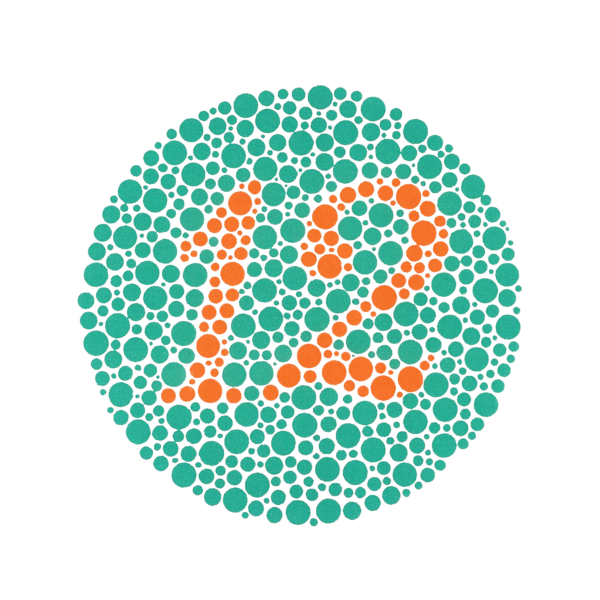
\includegraphics{Ishihara1.PNG}	    
% \end{figure}

\begin{figure}
\centering
\begin{subfigure}{.5\textwidth}
  \centering
  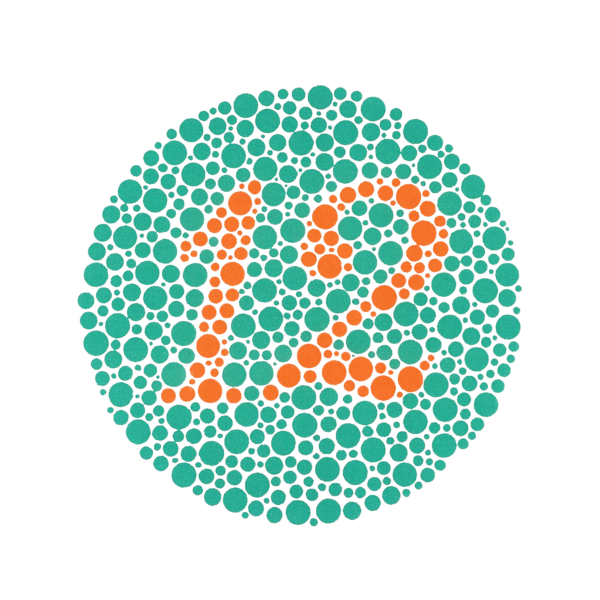
\includegraphics[width=.5\linewidth]{Ishihara1.PNG}
  \caption{Plate No. 1 (12)}
  \label{fig:sub1}
\end{subfigure}%
\begin{subfigure}{.5\textwidth}
  \centering
  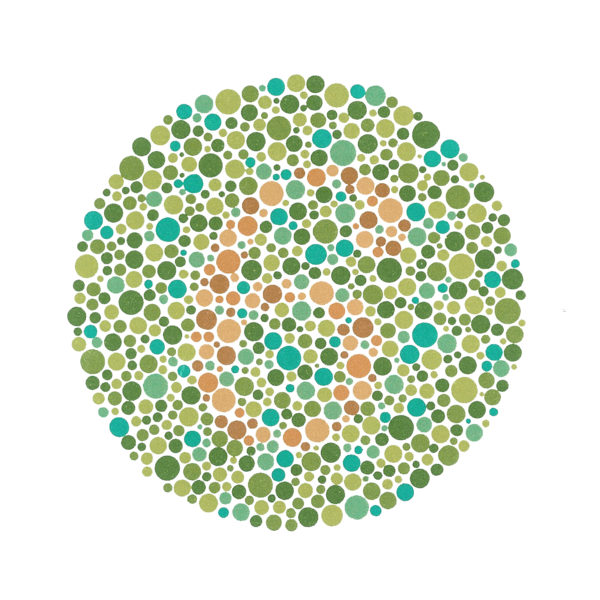
\includegraphics[width=.5\linewidth]{Ishihara2.PNG}
  \caption{Plate No. 13 (6)}
  \label{fig:sub2}
\end{subfigure}
\caption{Ishihara Test [Wikipedia]}
\label{fig:test}
\end{figure}

% {\vspace{10mm}}
% 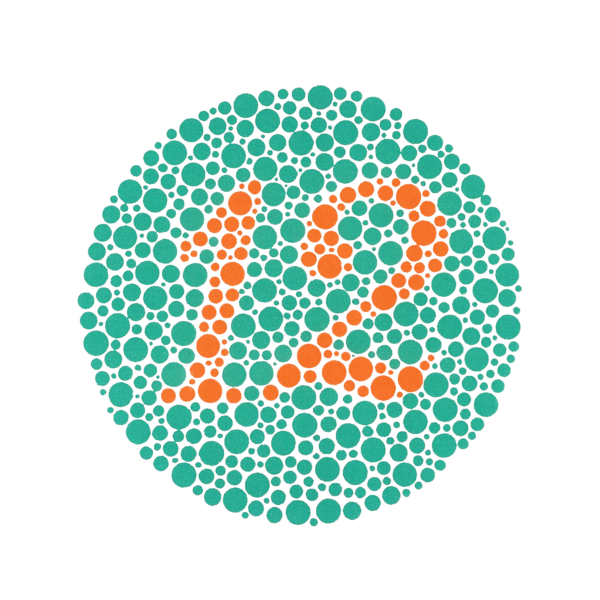
\includegraphics[width=0.4\linewidth]{Ishihara1.PNG}
% \captionof{figure}{Ishihara Plate No. 1 (12) [Wikipaedia]}


\section{Related Work}
\label{Related Work}

Quite a work has been done to both simulate and correct CVD. Ichikawa et al. [16sprweb] were the first publishers of a website recolouring tool that improves accessibility for people with CVD. Iaccarino et al. [15sprweb] proposed the use of edge services to recolour website images in transit to the user. ColorBlindnessSimulateCorrect by Seewald Solutions is one of the examples of an application developed to both simulate and correct CVD effect. It uses a linear transformation on rgb input. ‘Daltonize’ developed by www.daltonize.org can be used to recolor web pages. They first convert RGB values of a color to LMS values and then compensate for color blindness by shifting wavelengths away from the portion of the spectrum invisible to the dichromat, towards the visible portion.  Eyepilot [http://www.colorhelper.com/] enables computer users with red-green color blindness to decipher color-coded maps and graphs by letting the user place a floating window on top of any picture to distinguish among the various color fields. The GNOME[http://en.wikipedia.org/wiki/GNOME] desktop environment provides users with the option to switch a color filter on and off choosing from a set of possible color transformations that displace the colors in order to disambiguate them. While all these tools have proved to be effective in inducing differentiability in the content and thus providing legibility, but none of them have been able to retain the naturalness1, differentiability2 of the original web page.

One such tool which preserves naturalness and improves color differentiability is kuhn’s tool. One improvement on naturalness preservation was done by David et al. in SPRWeb[]. Which is also the basis of this thesis. SPRWeb performs better in preserving naturalness and differentiability than Kuhn’s tool. But it fails to make sure than all the foreground background color pairs have the minimum required contrast ratio threshold of 4.5 as per W3C guidelines.

\section{Definitions}
\label{Related Work}
\begin{itemize}
\item{\textbf{O}: } Original set of colors as parsed from CSS files associated with the webpage.
\item{\textbf{R}: } Replaced set of colors as computed by the recoloring algorithm. And obviously, size of \textbf{R} is always equal to size of \textbf{O}.
\item{\textbf{P}: } Number of color \textit{pairs} in a web page. A \textit{pair} of colors from a web page is of the form \textit{(fg,bg)}, where \textit{fg} is a foreground text color and \textit{bg} is a background color. There can be many such \textit{(fg,bg)} color pairs. 
\item{Naturalness[SPRweb]: } It is a measure of how close is set \textbf{R} to set \textbf{O}. Ideally, if our algorithm is able to find a set such that \textbf{R} = \textbf{O} then the naturalness will be maximum and the \textit{cost of naturalness} would be 0. \textit{Cost of naturalness} quantifies naturalness. We will define \textit{cost of naturalness} more precisely later in the document. 
\item{Inherited:} Inherited can further be classified in to three types:
\end{itemize}
